\documentclass[varwidth=true, border=2pt]{standalone}
\usepackage{tikz}

\begin{document}
    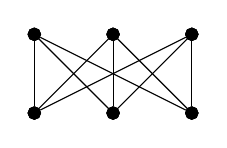
\begin{tikzpicture}
        \tikzstyle{point}=[circle,thick,draw=black,fill=black,inner sep=0pt,minimum width=4pt,minimum height=4pt]

        \foreach \x in {0,1,2}
        \foreach \y in {0,1,2}{
          \node (a)[point] at (\y,0) {};
          \node (b)[point] at (\x,1) {};
            \draw (a) -- (b);
        }
    \end{tikzpicture}
\end{document}
